%!Tex Root = ../Tutorat6.tex
% ./Packete.tex
% ./Design.tex
% ./Deklarationen.tex
% ./Aufgabe1.tex
% ./Aufgabe2.tex
% ./Bonus.tex

\section{Task 3}

\setcounter{task}{1}

\begin{frame}{Task 3}{Application control}
    \begin{tasknoinc}
        Consider the energy harvesting profile p(t) given in Figure 4 that repeats daily. What is the maximum average power $u_{max}$ that can be used by the system?
    \end{tasknoinc}
\end{frame}

\begin{frame}{Task 3}{Application control}
    \begin{solutionnoinc}
        \begin{figure}
            \centering
            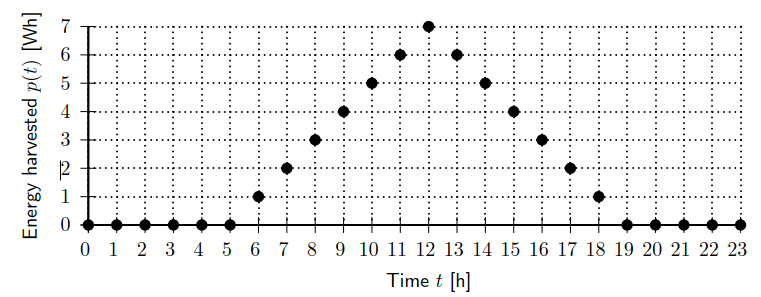
\includegraphics[scale=0.5]{figures/harvestingProfile.PNG}
        \end{figure}
    \end{solutionnoinc}
\end{frame}

\begin{frame}{Task 3}{Application control}
    \begin{solution}
        \begin{itemize}
            \item The daily harvested energy is calculated by: $(1Wh + 2Wh + 3Wh + 4Wh + 5H + 6Wh) * 2 + 7 Wh = 49Wh$
            \item This results in the following maximum average harvesting power: $u_{max} = \frac{49 Wh}{24h} = 2.04W$
        \end{itemize}
    \end{solution}
\end{frame}
\begin{frame}{Task 3}{Application control}
    \begin{tasknoinc}
        Given the knowledge of the daily energy input profile $p(t)$ in Figure 5, calculate the minimal battery size $B_{min}$ such that the used energy satisfies $u(t) = 2$ for every time interval during a day. Complete the diagram in Figure 6 with the daily evolution of the used energy $u(t)$ and the battery charge state $b(t)$ at the beginning of the interval for the found battery size $B_min$.
    \end{tasknoinc}
\end{frame}
\begin{frame}{Task 3}{Application control}
    \begin{solutionnoinc}
        \begin{itemize}
            \item The energy used during night, where the harvested energy is \alert{lower} than the consumed energy, is: $1Wh + 11 \cdot 2Wh + 1Wh = 24Wh$
            \item We need at least this much energy in our battery to compensate this deficit, meaning $B \geq 24Wh \Rightarrow B_{min} = 24Wh$.
        \end{itemize}
    \end{solutionnoinc}
\end{frame}
\begin{frame}[allowframebreaks]{Task 3}{Application control}
  \begin{solutionnoinc}
    \begin{figure}
        \centering
        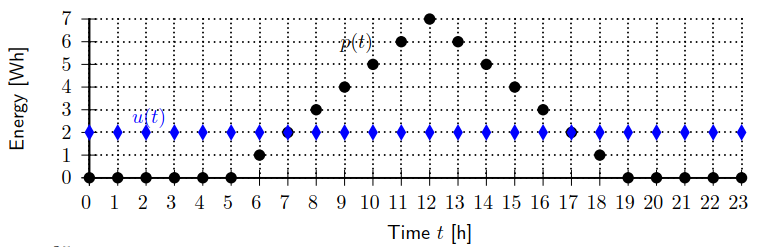
\includegraphics[scale=0.4]{figures/energyUsage_1.PNG}
    \end{figure}
  \end{solutionnoinc}
  \framebreak
  \begin{solution}
    \begin{figure}
        \centering
        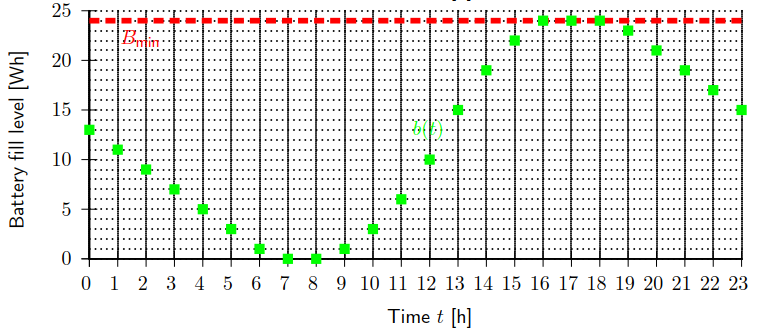
\includegraphics[scale=0.4]{figures/energyUsage_2.PNG}
    \end{figure}
  \end{solution}
  \begin{Sidenote}
    \begin{itemize}
      \item We observe that in intervals $t \in[0,6]$ and $t \in[18,23]$ of a day $u(t)>p(t)$ and therefore energy is used from the battery. In intervals $t \in[7,17]$ the battery is not used and the extra input power of intervals $t \in[8,16]$ is stored to the battery, with the battery overflowing in interval $t=16$.
    \end{itemize}
  \end{Sidenote}
\end{frame}
\begin{frame}[allowframebreaks]{Task 3}{}
  \begin{solutionnoinc}
    \begin{itemize}
      \item \alert{Step 1:} Maximize the minimum used energy
      \begin{itemize}
        \item increase all used energy values until battery size and correctness constraints not satisfied anymore
        \item to service the night we need $b(18)=11=B$
        \item battery depleted completely in between $[6, 7]$
        \item battery reaches full capacity of $11Wh$ around time $11$
        \item harvested energy wasted around time intervall $[11, 18]$, because it can't be stored
      \end{itemize}
    \item \alert{Step 2:} Increase the overall utility $\Rightarrow$ increase used energy $u(t)$ for $t\in [7, 17]$
        \begin{itemize}
          \item set the used energy $u(t) = 2$ for $t\in[7, 17]$
          \item conditions satisfied for $t\in [7, 17]$ $\checkmark$
            \begin{itemize}
              \item sufficient energy available in each time interval
              \item no superfluous energy as long as the battery is full
            \end{itemize}
          \item set the used energy $u(t) = 3$ for $t\in[8, 16]$
          \item same conditions still satisfied for $t\in [8, 16]$ $\checkmark$
          \item if $u(t)=4$ for $t\in[9, 15]$ then a full battery can't be reached anymore at $t=16$  $\times$
        \end{itemize}
      \end{itemize}
  \end{solutionnoinc}
  \begin{solutionnoinc}
    \begin{itemize}
      \item \alert{Step 3:} incrase energy up to a value that guarantees $b(16)=B$, determine appropriate value $u(t)$ to the the battery fully charged at this time by solving a equation for the time interval $[9, 15]$
      \begin{itemize}
        \item $(7-u)+2 \cdot(6-u)+2 \cdot(5-u)+2 \cdot(4-u)=11 \mathrm{Wh} \Rightarrow u=\frac{26}{7} \mathrm{Wh}$
        \item the resulting battery level is summarized in:
        \begin{figure}
          \centering
          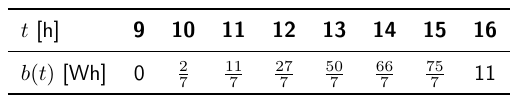
\includegraphics[width=0.6\textwidth]{./figures/task3_table.png}
        \end{figure}
      \end{itemize}
    \end{itemize}
  \end{solutionnoinc}
  \framebreak
  \begin{solutionnoinc}
    \begin{figure}
      \centering
      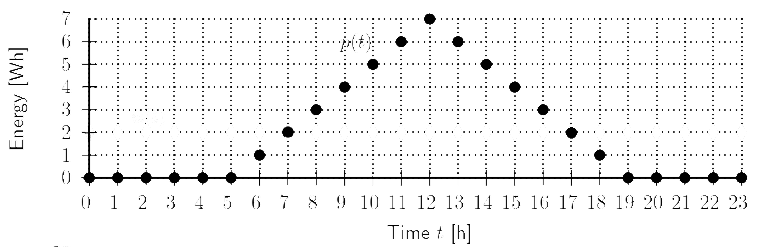
\includegraphics[width=0.6\textwidth]{./figures/energyUsage_1_empty.png}
    \end{figure}
  \end{solutionnoinc}
  \begin{solutionnoinc}
    \begin{figure}
      \centering
      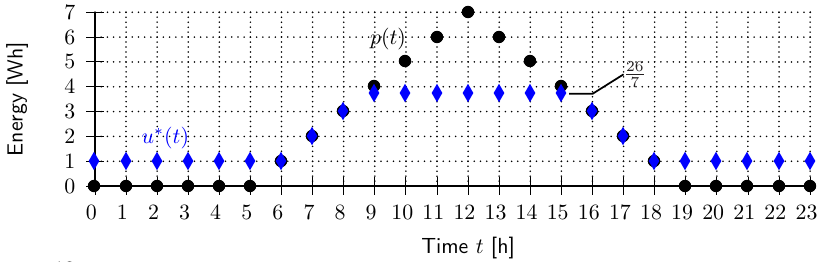
\includegraphics[width=\textwidth]{./figures/task3_use_and_harvest.png}
    \end{figure}
  \end{solutionnoinc}
  \begin{solution}
    \begin{figure}
      \centering
      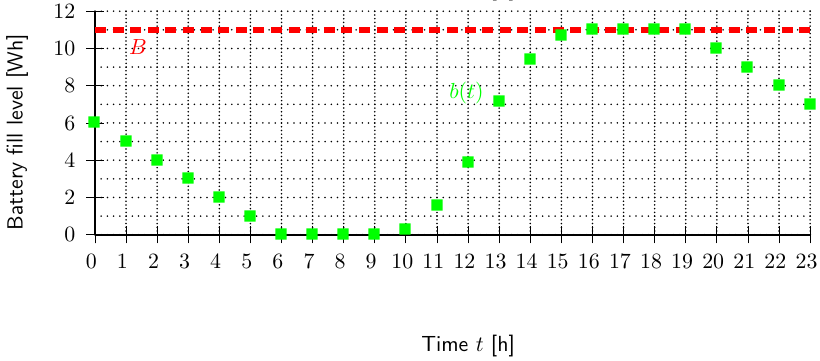
\includegraphics[width=\textwidth]{./figures/task3_battery.png}
    \end{figure}
  \end{solution}
  \framebreak
  \begin{tasknoinc}
    \begin{itemize}
      \item don't harvest any energy $p(t) = 0$ during one of the intervals $t\in[6, 18]$
      \item still same energy use $u^*(t)$ as computed a few slides above
      \item exact interval during which no energy is harvested is unknown
      \item determine consequences for all possible scenarios
    \end{itemize}
  \end{tasknoinc}
  \framebreak
  \begin{solution}
    \begin{itemize}
       \item If $p(t)=0$ for any interval $t \in[6,11]$, then there will be an immediate energy failure as the demand surpasses the available energy in the interval $[t, t+1]$.
      \item If $p(t)=0$ for any interval $t \in[12,18]$, the violation will happen some time during the night as the battery is not completely full in the afternoon.
    \end{itemize}
  \end{solution}
  \framebreak
  \begin{tasknoinc}
    \begin{itemize}
      \item use finite horizon control scheme for application control
      \item $p(12) = 0$ at time $t = 12$
    \end{itemize}
  \end{tasknoinc}
  \begin{solutionnoinc}
    \begin{itemize}
      \item for all times $t\le 12$ we have $\hat u^*(t) = u^*(t)$
      \item at time $t=13$ we have now $\hat b(t)= 4 - \frac{26}{7} + 5 - \frac{26}{7} + 6 - \frac{26}{7} - \frac{26}{7} =\frac{1}{7}$ instead of $\frac{50}{7}$
      \item new use function computed $u^*(t)$ which will determine the function $\hat u^*(t)$ from now on
      \item in order to achieve minimal used energy of $1Wh$ we need a full battery at $t=18$
      \item the new value of the used energy that guarantees a full battery level at t = 18 is computed while considering the energy balance equations for $t\in [13, 17]$:
      \begin{itemize}
        \item $\frac{1}{7}+(2-u)+(3-u)+(4-u)+(5-u)+(6-u)=11 \Rightarrow \hat{u}=\frac{64}{35} \approx 1.82 \mathrm{Wh}$
      \end{itemize}
      \item afterwards $\hat u^*(t)$ follows $u^*(t)$ as the battery state is identical to the one for use function $u^*(t)$ and there are no further mispredictions of the harvested energy $p(t)$
    \end{itemize}
  \end{solutionnoinc}
  \framebreak
  \begin{solutionnoinc}
    \begin{figure}
      \centering
      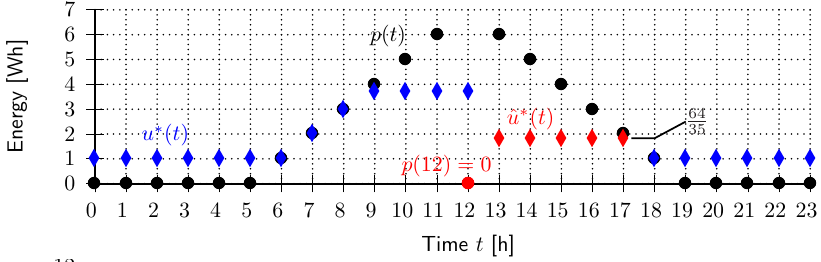
\includegraphics[width=\textwidth]{./figures/task5_use_and_harvest.png}
      \caption{The resulting energy use function $\hat u^*(t)$ and battery state $\hat b(t)$}
    \end{figure}
  \end{solutionnoinc}
  \begin{solutionnoinc}
    \begin{figure}
      \centering
      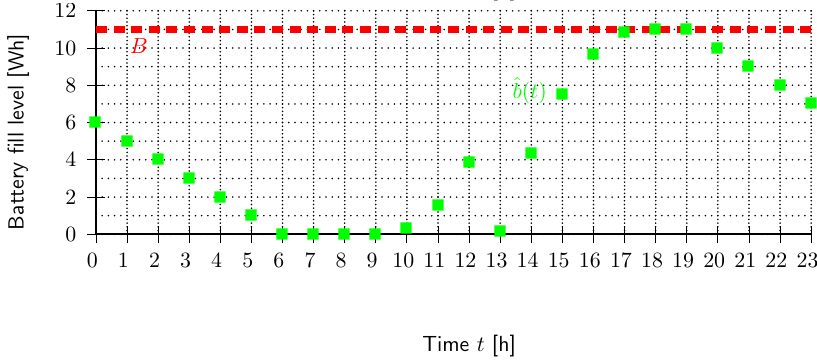
\includegraphics[width=0.7\textwidth]{./figures/task5_battery.png}
      \caption{The zero energy input at $t = 12$ results in a depleted battery at time $t = 13$. Consequently, the control scheme calculates an $\hat u^*(t)$ that is different from the initial $u^*(t)$ between $t \in [13, 17]$}
    \end{figure}
  \end{solutionnoinc}
\end{frame}
